% !TEX root = express.tex
The first contribution is about assessing the undecidability of the Generalised Synchronisability Problem for the \Mailbox semantics. 
This result strongly relies on the notion of accepting word.
Moreover, the entire section considers networks without any constraints on final configurations (\ie $\configFinal \subseteq \configSet$).  
%hence constraining the definition of network of communicating automata and the one of traces. For the former, we add a set $\finalGlobalStates$ of final states and traces are also modified in order to take into account only accepting executions. Namely, networks are now defined as $\Network = \left( (\Automaton{p})_{p \in \Part}, \messageSet, \finalGlobalStates\right)$, where $\finalGlobalStates$ is a set of tuples $(\state{s}{}{p})_{p\in P}$ such that $\state{s}{}{p} \in \finalStates{p}$. 
% We denote $\configFinal$ the set of configurations $\config = \left((\state{s}{}{p})_{p \in \Part}, \bufferSet\right)$ where $(\state{s}{}{p})_{p \in \Part} \in \finalGlobalStates$.
% The set of accepting executions and of traces are respectively:
% $$\accexecSet{\System{\Network}{\mailbox}{}} = \{\action_1\cdot\ \dots\ \cdot \action_n\ |\ \TransitionAsync{\configInit}{\action_1}{\config_1}{com}{}{} \TransitionAsync{}{\action_2}{}{com}{}{} \cdots \TransitionAsync{}{\action_n}{\config_n}{com}{}{}, \config_n  \in \configFinal\}, 
% $$
% $$\acctraceSet{\System{\Network}{\mailbox}{}} = \{\exec\projOut \mid \exec \in \accexecSet{\System{\Network}{com}{}}\}.$$
% The synchronisability problem then becomes 
% $\acctraceSet{\System{\Network}{\mailbox}{}} = \acctraceSet{\System{\Network}{\synch}{}}$. 
\paragraph{Post Correspondence Problem.}
We will resort to the Post Correspondence Problem (PCP) which is known to be an undecidable decision problem~\cite{post_variant_1946}, to prove that the Generalised Synchronisability Problem is undecidable. 
We will show that the encoding of a PCP instance \pcpinstance{} is not synchronisable if and only if the instance has a solution. 





% \begin{definition}[Word]\label{def:word}
%  Let $\Sigma$ an alphabet, a word $w= a_1a_2\dots a_n \in \Sigma^*$  is a finite sequence of symbols, such that $a_i \in \Sigma$,  for all $1 \leq i \leq n$.

% Let $w_a \in \Sigma^*$ and $w_b \in \Sigma^*$, 
% and $m,n \in \mathbb{N}$, such that  
% $w_a = w_{a,1}w_{a,2}\dots w_{a,m}$ and 
% $w_b = w_{b,1}w_{b,2}\dots w_{b,n}$. 
% The concatenation of $w_a$ and $w_b$, 
% written $w_a\cdot w_b$, 
% corresponds to the word $w_{a,1}w_{a,2}\dots w_{a,m}w_{b,1}w_{b,2}\dots w_{b,n}$. 
% %We denote $|w|$ the size of the word $w$.
% \end{definition} 

\begin{definition}[Post Correspondence Problem]\label{def:pcp}
Let $\alphabet$ be an alphabet with at least two symbols. An instance \pcpinstance{} of the PCP consists of two finite ordered lists of the same number of non-empty words $$\Word= {w_{1}, w_{2},\ldots , w_{n}}\text{ and }\text{\Word'}= {w'_{1}, w'_{2}, \ldots , w'_{n}}$$ such that $w_{i}, w'_{i} \in \alphabet^{*}$ for all indices $1 \leq i \leq n$. 
A solution of this instance is a finite sequence of indices $\Sol = ( i_{1}, i_{2}, \dots, i_{m} )$ with $m \geq 1$ and $i_{j} \in [1,n]$ for all $1 \leq j \leq m$ such that:
$$w_{i_{1}} \cdot w_{i_{2}} \cdot \ldots  \cdot w_{i_{m}} = w'_{i_{1}} \cdot w'_{i_{2}} \cdot \ldots  \cdot w'_{i_{m}} .$$
%We can represent the input as a set of $n$ blocks: 
%\begin{center}
%\begin{tabular}{c c c c}
%	$1$ & $2$ & & $n$ \\
%	\begin{tabular}{|c|}
%	\hline $w_{1}$ \\ \hline $w'_{1}$	\\ \hline 
%	\end{tabular}	
%&
%	\begin{tabular}{|c|}
%	\hline $w_{2}$ \\ \hline $w'_{2}$	\\ \hline
%	\end{tabular}
%&
%	\begin{tabular}{c}
%	\dots  \\ 	
%	\end{tabular}
%&
%	\begin{tabular}{|c|}
%	\hline $w_{n}$ \\ \hline $w'_{n}$	\\ \hline
%	\end{tabular} \\
%\end{tabular}
%\end{center}
\end{definition} 


\paragraph{Mailbox Encoding of the Post Correspondence Problem.}
The encoding in \Mailbox systems requires some care.
When an automaton is receiving messages from multiple participants, these messages are interleaved in the buffer and it is generally not possible to anticipate in which order these messages have been sent.

The encoding of an instance \pcpinstance{} of the PCP  is a parallel composition of four automata: $\Automaton{I}$, $\Automaton{W}$, $\Automaton{W'}$, and $\Automaton{L}$, where $\Automaton{I}$ sends the same indices to $\Automaton{W}$ and $\Automaton{W'}$ which in turn send the respective words to $\Automaton{L}$. $\Automaton{L}$ compare letters and, at the end of the run, its state allows to say if a solution exists. The topology and the buffer layout of the system is depicted in Figure~\ref{figure:topologyEncodeMail}. 

\begin{figure}[t]
	\centering
	\scalebox{0.9}{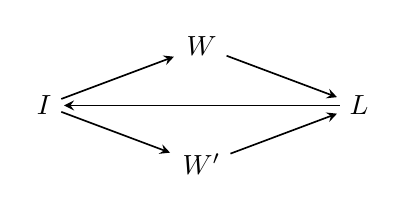
\begin{tikzpicture}[>=stealth,node distance=1.5cm,shorten >=1pt, every state/.style={text=black},semithick]
	\node (ai) at (-2,0) {$\Automaton{I}$};
	\node (aw) at (0,0.75) {$\Automaton{W}$};
	\node (awp) at (0,-0.75) {$\Automaton{W'}$};
	\node (al) at (2,0) {$\Automaton{L}$};
	\draw[->] (ai) -- (aw);
	\draw[->] (ai) -- (awp);
	\draw[->] (aw) -- (al);
	\draw[->] (awp) -- (al);
	\draw[->] (al) -- (ai);
\end{tikzpicture}}
	%%\includegraphics[scale = 0.1]{figures/encode_topo2.jpg}
	\caption{Topology of the encoding of an instance  \pcpinstance{} of the PCP} 
	\label{figure:topologyEncodeMail}
\end{figure}

We will explain our encoding over an example. Take the following PCP instance with  $\alphabet = \{a, b\}$,  $\Word = a, b, abab$ and $\Word' = ba, baa, b$. We know that there is a solution for this instance with $\Sol = (2, 1, 3)$. 
 Figures~\ref{figure:example:encodingMailAutBI}--\ref{figure:example:encodingMailAutBL} %to~\ref{figure:example:encodingMailAutBL} 
depict the automata solving the PCP instance.


%\begin{figure}[tp]
%	\begin{subfigure}{\textwidth}
%		\centering
%		\begin{tikzpicture}[>=stealth,node distance=1.5cm,shorten >=1pt,
    every state/.style={minimum size = 0pt},semithick]


      \node[state,initial,initial text={}]   at (0,0) (q0)  {$0$};
      \node[state] at (-1.5,1.7) (q1)  {$1$};
      \node[state] at (-1.5,-1.7) (q2)  {$2$};
      \node[state] at (1.5,-1.7) (q3)  {$3$};
      \node[state] at (2, 0) (qd)  {$\$$};
      \node[state, accepting] at (4, 0) (qd')  {$\$'$};
      
      
      
	\path (q0) edge[->, bend right = 10] node [sloped, above] {$\send{1}{I}{W}$} (q1);
	\path (q1) edge[->, bend right = 10] node [sloped, below] {$\send{1}{I}{W'}$} (q0);    
	
	\path (q0) edge[->, bend left=10] node [sloped, below] {$\send{2}{I}{W}$} (q2);
	\path (q2) edge[->, bend left=10] node [sloped, above] {$\send{2}{I}{W'}$} (q0);    
	
	\path (q0) edge[->, bend left=10] node [above,sloped] {$\send{3}{I}{W}$} (q3);
	\path (q3) edge[->, bend left=10] node [below, sloped] {$\send{3}{I}{W'}$} (q0);    
	
	\path (q0) edge[->] node [above] {$\send{\$}{I}{W}$} (qd);
	\path (qd) edge[->] node [above] {$\send{\$}{I}{W'}$} (qd');



		

\end{tikzpicture} 
%%		\scalebox{.8}{ \begin{tikzpicture}[>=stealth,node distance=1.5cm,shorten >=1pt,
    every state/.style={minimum size = 0pt},semithick]


      \node[state,initial,initial text={}]   at (0,0) (q0)  {$0$};
      \node[state] at (-1.5,1.7) (q1)  {$1$};
      \node[state] at (-1.5,-1.7) (q2)  {$2$};
      \node[state] at (1.5,-1.7) (q3)  {$3$};
      \node[state] at (2, 0) (qd)  {$\$$};
      \node[state, accepting] at (4, 0) (qd')  {$\$'$};
      
      
      
	\path (q0) edge[->, bend right = 10] node [sloped, above] {$\send{1}{I}{W}$} (q1);
	\path (q1) edge[->, bend right = 10] node [sloped, below] {$\send{1}{I}{W'}$} (q0);    
	
	\path (q0) edge[->, bend left=10] node [sloped, below] {$\send{2}{I}{W}$} (q2);
	\path (q2) edge[->, bend left=10] node [sloped, above] {$\send{2}{I}{W'}$} (q0);    
	
	\path (q0) edge[->, bend left=10] node [above,sloped] {$\send{3}{I}{W}$} (q3);
	\path (q3) edge[->, bend left=10] node [below, sloped] {$\send{3}{I}{W'}$} (q0);    
	
	\path (q0) edge[->] node [above] {$\send{\$}{I}{W}$} (qd);
	\path (qd) edge[->] node [above] {$\send{\$}{I}{W'}$} (qd');



		

\end{tikzpicture}  }
%		\caption{Automaton $\Automaton{I}$} 
%		\label{figure:example:encodingMailAutBI} 
%	\end{subfigure}
%%	\begin{subfigure}{.5\textwidth}
%%		\centering
%%		\scalebox{.7}{ \begin{tikzpicture}[>=stealth,node distance=1.5cm,shorten >=1pt,
    every state/.style={minimum size = 0pt}, semithick]


      \node[state,initial,initial text={}]   at (0,0) (q0)  {$0$};
      \node[state] at (2.5,1.5) (qa)  {$a$};
      \node[state] at (2.5,-1.5) (qb)  {$b$};
      \node[state] at (7,0) (q*)  {$*$};
      \node[state] at (3.5, 3.5) (qe)  {$e$};
      \node[state] at (6, 4) (qe')  {$e'$};
      \node[state, accepting] at (8, 4) (qok)  {$ok$};
      %\node[state, scale=0.8] at (12.8,4) (qokb) {};
      
	\path (q0) edge[->, bend left=10] node [above, sloped] {$\rec{a}{W}{L}$} (qa);
	\path (qa) edge[->, bend left=10] node [below, sloped] {$\rec{a}{W'}{L}$} (q0);    
	
	\path (q0) edge[->, bend left=10] node [above, sloped, pos = .6] {$\rec{b}{W}{L}$} (qb);
	\path (qb) edge[->, bend left=10] node [below, sloped] {$\rec{b}{W'}{L}$} (q0);    
	
	\path (q0) edge[->, bend left=40] node [left] {$\rec{end}{W}{L}$} (qe);
	\path (qe) edge[->] node [above] {$\rec{end}{W'}{L}$} (qe');
	\path (qe') edge[->] node [above] {$\send{ok}{L}{I}$} (qok);
	
	\path (q0) edge[->, bend right =90] node [below, scale = 0.9] 
		{\begin{tabular}{l l } 			
				$\rec{a}{W'}{L}$ & \\ 
				$\rec{b}{W'}{L}$ & $\rec{end}{W'}{L}$ \\ 
		\end{tabular}}	
	(q*); 
	
	\path (qb) edge[->, bend right =20] node [above, scale = 0.9, pos = .4] 
		{\begin{tabular}{l l} 
				$\rec{a}{W}{L}$ & $\rec{a}{W'}{L}$ \\ 
				$\rec{b}{W}{L}$  & $\rec{end}{W'}{L}$\\ 
				$\rec{end}{W}{L}$  \\ 
		\end{tabular}}	
	(q*); 
	
	\path (qa) edge[->, bend left =20] node [above, scale = 0.9] 
		{\begin{tabular}{l l} 
				$\rec{a}{W}{L}$ &   \\ 
				$\rec{b}{W}{L}$ &  $\rec{b}{W'}{L}$ \\ 
				$\rec{end}{W}{L}$ & $\rec{end}{W'}{L}$\\	
		\end{tabular}}	
	(q*); 
	
	\path (qe) edge[->, bend left =40] node [right, scale = 0.9] 
		{\begin{tabular}{l} 
				$\rec{a}{W'}{L}$  \\
				$\rec{b}{W'}{L}$  \\
				 \\
		\end{tabular}}	
	(q*); 
	
	\path (q*) edge[->, loop right ] node [right, scale = 0.9] {$*$}
		% {\begin{tabular}{l l} 
		% 		$\rec{a}{W}{L}$  & $\rec{a'}{W'}{L}$  \\
		% 		$\rec{b}{W}{L}$ & $\rec{b'}{W'}{L}$  \\
		% 		$\rec{end}{W}{L}$ & $\rec{end'}{W'}{L}$  \\
		% \end{tabular}}	
	(); 
	
		

\end{tikzpicture}  }
%%		\caption{Automaton $\Automaton{L}$} 
%%		\label{figure:example:encodingMailAutBL} 
%%	\end{subfigure}
%	\begin{subfigure}{\textwidth}
%		\centering
%		\begin{tikzpicture}[>=stealth,node distance=1.5cm,shorten >=1pt,
  every state/.style={minimum size = 0pt},semithick]


      \node[state,initial,initial text={}]   at (0.2,0) (q0)  {$0$};
      \node[state] at (2,2) (q10)  {$1,0$};
      \node[state] at (2,0) (q20)  {$2,0$};
      \node[state] at (2,-2) (q30)  {$3,0$};
      \node[state] at (4,-2) (q31)  {$3,1$};
      \node[state] at (6,-2) (q32)  {$3,2$};
      \node[state] at (8,-2) (q33)  {$3,3$};
      \node[state] at (6,0) (qf)  {$f$};
      \node[state] at (6,2) (qd)  {$\$$};
      \node[state, accepting] at (8,2) (qe)  {$e$};
      %\node[state, scale=0.8] at (15.2,0) (qeb) {};
      
    
    \path (q0) edge[->, bend left] node [left] {$\rec{1}{I}{W}$} (q10);
    \path (q0) edge[->] node [above] {$\rec{2}{I}{W}$} (q20);
    \path (q0) edge[->, bend right] node [left] {$\rec{3}{I}{W}$} (q30);

    \path (q10) edge[->, bend left=25] node [sloped, above] {$\send{a}{W}{L}$} (qf);
    \path (qf) edge[->] node [sloped, above] {$\rec{1}{I}{W}$} (q10);

    \path (q20) edge[->, bend left=10] node [sloped, above] {$\send{b}{W}{L}$} (qf);
    \path (qf) edge[->, bend left=10] node [sloped, below] {$\rec{2}{I}{W}$} (q20);
    
    \path (q30) edge[->] node [below] {$\send{a}{W}{L}$} (q31);
    \path (q31) edge[->] node [below] {$\send{b}{W}{L}$} (q32);
    \path (q32) edge[->] node [below] {$\send{a}{W}{L}$} (q33);
    \path (q33) edge[->, bend right] node [sloped, above] {$\send{b}{W}{L}$} (qf);
    \path (qf) edge[->, bend right=5] node [pos = .3, sloped, below] {$\rec{3}{I}{W}$} (q30);
    
    \path (qf) edge[->] node [right] {$\rec{\$}{I}{W}$} (qd);
    \path (qd) edge[->] node [above] {$\send{end}{W}{L}$} (qe);


\end{tikzpicture} 
%%		\scalebox{.8}{\begin{tikzpicture}[>=stealth,node distance=1.5cm,shorten >=1pt,
  every state/.style={minimum size = 0pt},semithick]


      \node[state,initial,initial text={}]   at (0.2,0) (q0)  {$0$};
      \node[state] at (2,2) (q10)  {$1,0$};
      \node[state] at (2,0) (q20)  {$2,0$};
      \node[state] at (2,-2) (q30)  {$3,0$};
      \node[state] at (4,-2) (q31)  {$3,1$};
      \node[state] at (6,-2) (q32)  {$3,2$};
      \node[state] at (8,-2) (q33)  {$3,3$};
      \node[state] at (6,0) (qf)  {$f$};
      \node[state] at (6,2) (qd)  {$\$$};
      \node[state, accepting] at (8,2) (qe)  {$e$};
      %\node[state, scale=0.8] at (15.2,0) (qeb) {};
      
    
    \path (q0) edge[->, bend left] node [left] {$\rec{1}{I}{W}$} (q10);
    \path (q0) edge[->] node [above] {$\rec{2}{I}{W}$} (q20);
    \path (q0) edge[->, bend right] node [left] {$\rec{3}{I}{W}$} (q30);

    \path (q10) edge[->, bend left=25] node [sloped, above] {$\send{a}{W}{L}$} (qf);
    \path (qf) edge[->] node [sloped, above] {$\rec{1}{I}{W}$} (q10);

    \path (q20) edge[->, bend left=10] node [sloped, above] {$\send{b}{W}{L}$} (qf);
    \path (qf) edge[->, bend left=10] node [sloped, below] {$\rec{2}{I}{W}$} (q20);
    
    \path (q30) edge[->] node [below] {$\send{a}{W}{L}$} (q31);
    \path (q31) edge[->] node [below] {$\send{b}{W}{L}$} (q32);
    \path (q32) edge[->] node [below] {$\send{a}{W}{L}$} (q33);
    \path (q33) edge[->, bend right] node [sloped, above] {$\send{b}{W}{L}$} (qf);
    \path (qf) edge[->, bend right=5] node [pos = .3, sloped, below] {$\rec{3}{I}{W}$} (q30);
    
    \path (qf) edge[->] node [right] {$\rec{\$}{I}{W}$} (qd);
    \path (qd) edge[->] node [above] {$\send{end}{W}{L}$} (qe);


\end{tikzpicture} }
%		\caption{Automaton $\Automaton{W}$} 
%		\label{figure:example:encodingMailAutBW}
%	\end{subfigure}
%	\begin{subfigure}{\textwidth}
%		\centering
%		\begin{tikzpicture}[>=stealth,node distance=1.5cm,shorten >=1pt,
  every state/.style={minimum size = 0pt},semithick]

      \node[state,initial,initial text={}]   at (0.1,0) (q0)  {$0$};
      \node[state] at (2,2) (q10)  {$1,0$};
      \node[state] at (4.1, 2) (q11) {$1,1$};
      \node[state] at (2,-2) (q20)  {$2,0$};
      \node[state] at (4.1, -2) (q21) {$2,1$};
      \node[state] at (6.5, -2) (q22) {$2,2$};
      \node[state] at (2,0)  (q30)  {$3,0$};
      \node[state] at (6.5,0) (qf)  {$f$};
      \node[state] at (6.5,2) (qd)  {$\$$};
      \node[state, accepting] at (8.7,2) (qe)  {$e$};
      %\node[state, scale=0.8] at (15.4,0) (qeb) {};
      
    
    \path (q0) edge[->, bend left] node [left] {$\rec{1}{I}{W'}$} (q10);
    \path (q0) edge[->, bend right] node [left] {$\rec{2}{I}{W'}$} (q20);
    \path (q0) edge[->] node [above] {$\rec{3}{I}{W'}$} (q30);

    \path (q10) edge[->] node [above] {$\send{b}{W'}{L}$} (q11);
    \path (q11) edge[->, bend left = 15] node [above, sloped] {$\send{a}{W'}{L}$} (qf);
    \path (qf) edge[->, bend left = 5] node [above, sloped] {$\rec{1}{I}{W'}$} (q10);
    
    \path (q20) edge[->] node [sloped, below] {$\send{b}{W'}{L}$} (q21);
    \path (q21) edge[->] node [below] {$\send{a}{W'}{L}$} (q22);
    \path (q22) edge[->] node [right] {$\send{a}{W'}{L}$} (qf);
    \path (qf) edge[->, bend right=5] node [below, sloped] {$\rec{2}{I}{W'}$} (q20);
    
    
    \path (q30) edge[->, bend left = 5] node [above, sloped, pos= .4] {$\send{b}{W'}{L}$} (qf);
    \path (qf) edge[->, bend left = 5] node [below, sloped, pos = .6] {$\rec{3}{I}{W'}$} (q30);
    
    \path (qf) edge[->] node [right] {$\rec{\$}{I}{W'}$} (qd);
    \path (qd) edge[->] node [above] {$\send{end}{W'}{L}$} (qe);

\end{tikzpicture} 
%%		\scalebox{.8}{ \begin{tikzpicture}[>=stealth,node distance=1.5cm,shorten >=1pt,
  every state/.style={minimum size = 0pt},semithick]

      \node[state,initial,initial text={}]   at (0.1,0) (q0)  {$0$};
      \node[state] at (2,2) (q10)  {$1,0$};
      \node[state] at (4.1, 2) (q11) {$1,1$};
      \node[state] at (2,-2) (q20)  {$2,0$};
      \node[state] at (4.1, -2) (q21) {$2,1$};
      \node[state] at (6.5, -2) (q22) {$2,2$};
      \node[state] at (2,0)  (q30)  {$3,0$};
      \node[state] at (6.5,0) (qf)  {$f$};
      \node[state] at (6.5,2) (qd)  {$\$$};
      \node[state, accepting] at (8.7,2) (qe)  {$e$};
      %\node[state, scale=0.8] at (15.4,0) (qeb) {};
      
    
    \path (q0) edge[->, bend left] node [left] {$\rec{1}{I}{W'}$} (q10);
    \path (q0) edge[->, bend right] node [left] {$\rec{2}{I}{W'}$} (q20);
    \path (q0) edge[->] node [above] {$\rec{3}{I}{W'}$} (q30);

    \path (q10) edge[->] node [above] {$\send{b}{W'}{L}$} (q11);
    \path (q11) edge[->, bend left = 15] node [above, sloped] {$\send{a}{W'}{L}$} (qf);
    \path (qf) edge[->, bend left = 5] node [above, sloped] {$\rec{1}{I}{W'}$} (q10);
    
    \path (q20) edge[->] node [sloped, below] {$\send{b}{W'}{L}$} (q21);
    \path (q21) edge[->] node [below] {$\send{a}{W'}{L}$} (q22);
    \path (q22) edge[->] node [right] {$\send{a}{W'}{L}$} (qf);
    \path (qf) edge[->, bend right=5] node [below, sloped] {$\rec{2}{I}{W'}$} (q20);
    
    
    \path (q30) edge[->, bend left = 5] node [above, sloped, pos= .4] {$\send{b}{W'}{L}$} (qf);
    \path (qf) edge[->, bend left = 5] node [below, sloped, pos = .6] {$\rec{3}{I}{W'}$} (q30);
    
    \path (qf) edge[->] node [right] {$\rec{\$}{I}{W'}$} (qd);
    \path (qd) edge[->] node [above] {$\send{end}{W'}{L}$} (qe);

\end{tikzpicture}  }
%		\caption{Automaton $\Automaton{W'}$} 
%		\label{figure:example:encodingMailAutBWb} 
%	\end{subfigure}
%	\caption{Network $\Encode{\Word,\Word'}{\mailbox}$}
%	\label{figure:example:encodingMail}
%\end{figure}


Automaton $\Automaton{I}$ guesses the sequence of indexes and sends it to both $\Automaton{W}$ and $\Automaton{W'}$. The message $\$$ is used to signal the end of the sequence.
Automaton $\Automaton{W}$ and  $\Automaton{W'}$ receive indexes  from $\Automaton{I}$ and send the corresponding sequences of letters to $\Automaton{L}$. At the reception of message $\$$, they send messages $end$ to $\Automaton{L}$.
%The primed version of the letters is used to distinguish whether the letter is produced by $\Automaton{W}$ or $\Automaton{W'}$.  
Automaton $\Automaton{L}$ checks whether the sequences of letters produced by $\Automaton{W}$ and $\Automaton{W'}$ coincide. Letters from  $\Automaton{W}$ and $\Automaton{W'}$ need to be alternate and are read in turn, and the additional receptions are used to make the system synchronisable and to recognize errors (\ie sequences that are not a solution).
If all comparisons succeed, included the  $end$  messages, then $\Automaton{L}$  sends message $ok$ that is not received by any participant and ends up in the unique accepting state.

More formally, we define the encoding as follows. 
\begin{definition}[Encoding of PCP in mailbox system]\label{def:encodingMail}
 Let $(\Word,\Word')$ be a PCP instance over $\alphabet$. 
 %where \mbox{$\Word = w_1, \ldots, w_n$} and $\Word'=w'_1, \dots, w'_n$. 
The encoding of $(\Word,\Word')$ is the network $\Encode{\Word,\Word'}{\mailbox} =  \left((\Automaton{p})_{p \in \Part}, \messageSet\right)$ where:
\begin{itemize}
	\item $\Part = \left\{ I, W, W', L\right\} $
	\item $\messageSet = \left\{ \msg{i}{I}{W}, \msg{i}{I}{W'} \mid i \in [1,n]\right\} \cup \left\{ \msg{\alpha}{W}{L},\msg{\alpha}{W'}{L} \mid \alpha \in \Sigma \right\} \cup M $ with\\
		$ M = \left\{ \msg{\$}{I}{W}, \msg{\$}{I}{W'}, \msg{end}{W}{L}, \msg{end}{W'}{L}, \msg{ok}{L}{I}\right\} $
\begin{figure}[t]
	\centering
	\begin{tikzpicture}[>=stealth,node distance=1.5cm,shorten >=1pt,
    every state/.style={minimum size = 0pt},semithick]


      \node[state,initial,initial text={}]   at (0,0) (q0)  {$0$};
      \node[state] at (-1.5,1.7) (q1)  {$1$};
      \node[state] at (-1.5,-1.7) (q2)  {$2$};
      \node[state] at (1.5,-1.7) (q3)  {$3$};
      \node[state] at (2, 0) (qd)  {$\$$};
      \node[state, accepting] at (4, 0) (qd')  {$\$'$};
      
      
      
	\path (q0) edge[->, bend right = 10] node [sloped, above] {$\send{1}{I}{W}$} (q1);
	\path (q1) edge[->, bend right = 10] node [sloped, below] {$\send{1}{I}{W'}$} (q0);    
	
	\path (q0) edge[->, bend left=10] node [sloped, below] {$\send{2}{I}{W}$} (q2);
	\path (q2) edge[->, bend left=10] node [sloped, above] {$\send{2}{I}{W'}$} (q0);    
	
	\path (q0) edge[->, bend left=10] node [above,sloped] {$\send{3}{I}{W}$} (q3);
	\path (q3) edge[->, bend left=10] node [below, sloped] {$\send{3}{I}{W'}$} (q0);    
	
	\path (q0) edge[->] node [above] {$\send{\$}{I}{W}$} (qd);
	\path (qd) edge[->] node [above] {$\send{\$}{I}{W'}$} (qd');



		

\end{tikzpicture} 
	\caption{Automaton $\Automaton{I}$} 
	\label{figure:example:encodingMailAutBI}
\end{figure}
	\item  $\Automaton{I} = (\stateSet{I}, \state{s}{0}{I}, \messageSet, \rightarrow_I, \finalStates{\Automaton{I}} )$ where $\stateSet{I} = \left\{\state{q}{0}{}, \state{q}{\$}{}, \state{q}{\$'}{}\right\} \cup \left\{ \state{q}{i}{} \mid i \in [1,n] \right\}$, $\state{s}{0}{I} = \state{q}{0}{}$, $\finalStates{\Automaton{I}} = \Set{\state{q}{\$'}{}}$ and 
		$$ 
		\rightarrow_I  = \ \left\{ \TransitionAsync
					{\state{q}{0}{}}
					{\send{i}{I}{W}}
					{\state{q}{i}{}}{}{},
					\TransitionAsync	
					{\state{q}{i}{}}
					{\send{i}{I}{W'}}
					{\state{q}{0}{}}{}{}			
					\mid i \in [1,n]\right\} 
		 \cup \left\{ \TransitionAsync
					{\state{q}{0}{}}
					{\send{\$}{I}{W}}
					{\state{q}{\$}{}}{}{},
		 \TransitionAsync
					{\state{q}{\$}{}}
					{\send{\$}{I}{W'}}
					{\state{q}{\$'}{}}{}{} \right\} $$
\begin{figure}[t]
	\centering
	\begin{tikzpicture}[>=stealth,node distance=1.5cm,shorten >=1pt,
  every state/.style={minimum size = 0pt},semithick]


      \node[state,initial,initial text={}]   at (0.2,0) (q0)  {$0$};
      \node[state] at (2,2) (q10)  {$1,0$};
      \node[state] at (2,0) (q20)  {$2,0$};
      \node[state] at (2,-2) (q30)  {$3,0$};
      \node[state] at (4,-2) (q31)  {$3,1$};
      \node[state] at (6,-2) (q32)  {$3,2$};
      \node[state] at (8,-2) (q33)  {$3,3$};
      \node[state] at (6,0) (qf)  {$f$};
      \node[state] at (6,2) (qd)  {$\$$};
      \node[state, accepting] at (8,2) (qe)  {$e$};
      %\node[state, scale=0.8] at (15.2,0) (qeb) {};
      
    
    \path (q0) edge[->, bend left] node [left] {$\rec{1}{I}{W}$} (q10);
    \path (q0) edge[->] node [above] {$\rec{2}{I}{W}$} (q20);
    \path (q0) edge[->, bend right] node [left] {$\rec{3}{I}{W}$} (q30);

    \path (q10) edge[->, bend left=25] node [sloped, above] {$\send{a}{W}{L}$} (qf);
    \path (qf) edge[->] node [sloped, above] {$\rec{1}{I}{W}$} (q10);

    \path (q20) edge[->, bend left=10] node [sloped, above] {$\send{b}{W}{L}$} (qf);
    \path (qf) edge[->, bend left=10] node [sloped, below] {$\rec{2}{I}{W}$} (q20);
    
    \path (q30) edge[->] node [below] {$\send{a}{W}{L}$} (q31);
    \path (q31) edge[->] node [below] {$\send{b}{W}{L}$} (q32);
    \path (q32) edge[->] node [below] {$\send{a}{W}{L}$} (q33);
    \path (q33) edge[->, bend right] node [sloped, above] {$\send{b}{W}{L}$} (qf);
    \path (qf) edge[->, bend right=5] node [pos = .3, sloped, below] {$\rec{3}{I}{W}$} (q30);
    
    \path (qf) edge[->] node [right] {$\rec{\$}{I}{W}$} (qd);
    \path (qd) edge[->] node [above] {$\send{end}{W}{L}$} (qe);


\end{tikzpicture} 
	\caption{Automaton $\Automaton{W}$} 
	\label{figure:example:encodingMailAutBW}
\end{figure}
\begin{figure}[t]
	\centering
	\begin{tikzpicture}[>=stealth,node distance=1.5cm,shorten >=1pt,
  every state/.style={minimum size = 0pt},semithick]

      \node[state,initial,initial text={}]   at (0.1,0) (q0)  {$0$};
      \node[state] at (2,2) (q10)  {$1,0$};
      \node[state] at (4.1, 2) (q11) {$1,1$};
      \node[state] at (2,-2) (q20)  {$2,0$};
      \node[state] at (4.1, -2) (q21) {$2,1$};
      \node[state] at (6.5, -2) (q22) {$2,2$};
      \node[state] at (2,0)  (q30)  {$3,0$};
      \node[state] at (6.5,0) (qf)  {$f$};
      \node[state] at (6.5,2) (qd)  {$\$$};
      \node[state, accepting] at (8.7,2) (qe)  {$e$};
      %\node[state, scale=0.8] at (15.4,0) (qeb) {};
      
    
    \path (q0) edge[->, bend left] node [left] {$\rec{1}{I}{W'}$} (q10);
    \path (q0) edge[->, bend right] node [left] {$\rec{2}{I}{W'}$} (q20);
    \path (q0) edge[->] node [above] {$\rec{3}{I}{W'}$} (q30);

    \path (q10) edge[->] node [above] {$\send{b}{W'}{L}$} (q11);
    \path (q11) edge[->, bend left = 15] node [above, sloped] {$\send{a}{W'}{L}$} (qf);
    \path (qf) edge[->, bend left = 5] node [above, sloped] {$\rec{1}{I}{W'}$} (q10);
    
    \path (q20) edge[->] node [sloped, below] {$\send{b}{W'}{L}$} (q21);
    \path (q21) edge[->] node [below] {$\send{a}{W'}{L}$} (q22);
    \path (q22) edge[->] node [right] {$\send{a}{W'}{L}$} (qf);
    \path (qf) edge[->, bend right=5] node [below, sloped] {$\rec{2}{I}{W'}$} (q20);
    
    
    \path (q30) edge[->, bend left = 5] node [above, sloped, pos= .4] {$\send{b}{W'}{L}$} (qf);
    \path (qf) edge[->, bend left = 5] node [below, sloped, pos = .6] {$\rec{3}{I}{W'}$} (q30);
    
    \path (qf) edge[->] node [right] {$\rec{\$}{I}{W'}$} (qd);
    \path (qd) edge[->] node [above] {$\send{end}{W'}{L}$} (qe);

\end{tikzpicture} 
	\caption{Automaton $\Automaton{W'}$} 
	\label{figure:example:encodingMailAutBWb}
\end{figure}
	\item  $\Automaton{W} = (S_W, \state{s}{0}{W}, \messageSet, \rightarrow_W, \finalStates{\Automaton{W}})$ where 
$S_W  = \left\{\state{q}{0}{}, \state{q}{f}{}, \state{q}{\$}{}, \state{q}{e}{}\right\} \cup\left\{q_{i,j} \mid i \in [1,n] \wedge j \in [0, \length{w_i}-1 ] \right\}$,\linebreak $\state{s}{0}{W}  = \state{q}{0}{}$, $\finalStates{\Automaton{W}} = \Set{\state{q}{e}{}}$ and 
		\begin{align*}
		 \rightarrow_W ={}& \left\{ \Transition
				{\state{q}{0}{}}
				{\rec{i}{I}{W}}
				{\state{q}{i,0}{}}
				{},
				\Transition
				{\state{q}{f}{}}
				{\rec{i}{I}{W}}
				{\state{q}{i,0}{}}
				{}
				\mid i \in [1,n] \right\}  
		 \cup \left\{ \Transition
				{\state{q}{i,|w_i|-1}{}}
				{\send{\alpha}{W}{L}}
				{\state{q}{f}{}}
				{} \mid \alpha = w_{i,|w_i|} \wedge i \in [1,n] \right\}  \\ 
		&{}\cup \left\{ \Transition
				{\state{q}{i,j}{}}
				{\send{\alpha}{W}{L}}
				{\state{q}{i,j+1}{}}
				{}\mid   \alpha = w_{i,j+1} \wedge i \in [1,n] \wedge j \in [1, |w_i|-2]  \right\}\\ 
		&{}\cup \left\{ \Transition
				{\state{q}{f}{}}
				{\rec{\$}{I}{W}}
				{\state{q}{\$}{}}
				{}, \Transition
				{\state{q}{\$}{}}
				{\send{end}{W}{L}}
				{\state{q}{e}{}}
				{} \right\}
		\end{align*}
\begin{figure}[t]
	\centering
	\begin{tikzpicture}[>=stealth,node distance=1.5cm,shorten >=1pt,
    every state/.style={minimum size = 0pt}, semithick]


      \node[state,initial,initial text={}]   at (0,0) (q0)  {$0$};
      \node[state] at (2.5,1.5) (qa)  {$a$};
      \node[state] at (2.5,-1.5) (qb)  {$b$};
      \node[state] at (7,0) (q*)  {$*$};
      \node[state] at (3.5, 3.5) (qe)  {$e$};
      \node[state] at (6, 4) (qe')  {$e'$};
      \node[state, accepting] at (8, 4) (qok)  {$ok$};
      %\node[state, scale=0.8] at (12.8,4) (qokb) {};
      
	\path (q0) edge[->, bend left=10] node [above, sloped] {$\rec{a}{W}{L}$} (qa);
	\path (qa) edge[->, bend left=10] node [below, sloped] {$\rec{a}{W'}{L}$} (q0);    
	
	\path (q0) edge[->, bend left=10] node [above, sloped, pos = .6] {$\rec{b}{W}{L}$} (qb);
	\path (qb) edge[->, bend left=10] node [below, sloped] {$\rec{b}{W'}{L}$} (q0);    
	
	\path (q0) edge[->, bend left=40] node [left] {$\rec{end}{W}{L}$} (qe);
	\path (qe) edge[->] node [above] {$\rec{end}{W'}{L}$} (qe');
	\path (qe') edge[->] node [above] {$\send{ok}{L}{I}$} (qok);
	
	\path (q0) edge[->, bend right =90] node [below, scale = 0.9] 
		{\begin{tabular}{l l } 			
				$\rec{a}{W'}{L}$ & \\ 
				$\rec{b}{W'}{L}$ & $\rec{end}{W'}{L}$ \\ 
		\end{tabular}}	
	(q*); 
	
	\path (qb) edge[->, bend right =20] node [above, scale = 0.9, pos = .4] 
		{\begin{tabular}{l l} 
				$\rec{a}{W}{L}$ & $\rec{a}{W'}{L}$ \\ 
				$\rec{b}{W}{L}$  & $\rec{end}{W'}{L}$\\ 
				$\rec{end}{W}{L}$  \\ 
		\end{tabular}}	
	(q*); 
	
	\path (qa) edge[->, bend left =20] node [above, scale = 0.9] 
		{\begin{tabular}{l l} 
				$\rec{a}{W}{L}$ &   \\ 
				$\rec{b}{W}{L}$ &  $\rec{b}{W'}{L}$ \\ 
				$\rec{end}{W}{L}$ & $\rec{end}{W'}{L}$\\	
		\end{tabular}}	
	(q*); 
	
	\path (qe) edge[->, bend left =40] node [right, scale = 0.9] 
		{\begin{tabular}{l} 
				$\rec{a}{W'}{L}$  \\
				$\rec{b}{W'}{L}$  \\
				 \\
		\end{tabular}}	
	(q*); 
	
	\path (q*) edge[->, loop right ] node [right, scale = 0.9] {$*$}
		% {\begin{tabular}{l l} 
		% 		$\rec{a}{W}{L}$  & $\rec{a'}{W'}{L}$  \\
		% 		$\rec{b}{W}{L}$ & $\rec{b'}{W'}{L}$  \\
		% 		$\rec{end}{W}{L}$ & $\rec{end'}{W'}{L}$  \\
		% \end{tabular}}	
	(); 
	
		

\end{tikzpicture} 
	\caption{Automaton $\Automaton{L}$} 
	\label{figure:example:encodingMailAutBL} 
\end{figure}
	\item $\Automaton{L} = (S_L, \state{s}{0}{L}, M, \rightarrow_L, \finalStates{\Automaton{L}})$ where $S_L = \{\state{q}{0}{}, \state{q}{e}{}, \state{q}{e'}{}, \state{q}{ok}{}, \state{q}{*}{}\} \cup \{\state{q}{\alpha}{} | \alpha \in \Sigma \}$, $\state{s}{0}{L} = \state{q}{0}{}$, $\finalStates{\Automaton{L}} = \Set{\state{q}{ok}{}}$ and 
		\begin{align*} \rightarrow_L =
		&\ \left\{ \Transition
				{\state{q}{0}{}}
				{\rec{\alpha}{W}{L}}
				{\state{q}{\alpha}{}}
				{},
				\Transition
				{\state{q}{\alpha}{}}
				{\rec{\alpha}{W'}{L}}
				{\state{q}{0}{}}
				{}\mid \alpha \in \Sigma \right\}   
		 \cup \left\{ \Transition
				{\state{q}{\alpha}{}}
				{\rec{\beta}{W'}{L}}
				{\state{q}{*}{}}
				{}\mid \beta \in \Sigma \cup \{end\} \wedge \beta \neq \alpha \right\} \\%
		&\ \cup \left\{ 
				 \Transition
				{\state{q}{0}{}}
				{\rec{\alpha}{W'}{L}}
				{\state{q}{*}{}}
				{} \mid \alpha \in \Sigma \cup \{end\}\right\} \cup
				\left\{
				\Transition
				{\state{q}{\alpha}{}}
				{\rec{\beta}{W}{L}}
				{\state{q}{*}{}}
				{} \mid \beta \in \Sigma \cup \{end\} \right\} \\ 
		&\ \cup \left\{ \Transition
				{\state{q}{e}{}}
				{\rec{\alpha}{W}{L}}
				{\state{q}{*}{}}
				{}\ |\ \alpha \in \Sigma \right\} \cup \left\{ \Transition
				{\state{q}{e}{}}
				{\rec{\alpha}{W'}{L}}
				{\state{q}{*}{}}
				{}\ |\ \alpha \in \Sigma \right\} \\ 
		&\ \cup \left\{ \Transition
				{\state{q}{*}{}}
				{\rec{\alpha}{X}{L}}
				{\state{q}{*}{}}
				{}\ |\ \alpha \in \Sigma \cup \{end\} \wedge X \in \{W, W'\}\right\} \\ 
		&\ \cup \left\{  
				\Transition
				{\state{q}{0}{}}
				{\rec{end}{W}{L}}
				{\state{q}{e}{}}
				{},
				 \Transition
				{\state{q}{e}{}}
				{\rec{end}{W'}{I}}
				{\state{q}{e'}{}}
				{}, 
				\Transition
				{\state{q}{e'}{}}
				{\send{ok}{L}{I}}
				{\state{q}{ok}{}}
				{} \right\}
		\end{align*}
%\item $F = \{(\state{q}{\$'}{I}, \state{q}{e}{W},\state{q}{e}{W'}, \state{q}{ok}{L})\}$.
\end{itemize}
$\Automaton{W'}$ is defined as $\Automaton{W}$ but considering $\Word'$ instead of $\Word$. 
\end{definition}

It is easy to see that in the synchronous semantics the system cannot reach any final configuration, because of message $ok$ which cannot be sent since it cannot be received. The set of traces of the synchronous system is indeed empty. 

 \begin{lemma}  \label{lem:emptyMail}
Let \pcpinstance{} an instance of PCP and $\Network  = \Encode{\Word,\Word'}{\mailbox}$ its encoding into communicating automata. Then $\traceSet{\System{\Network}{\synch}{}} = \emptyset$.
 \end{lemma} 

In the \Mailbox semantics, message $ok$ can be sent only if the encoded instance of PCP has a solution.
If the instance of PCP has no solution, then the \Mailbox system is unable to reach the final configuration and the set of traces is empty.
Summing up, the set of traces is not empty if and  only if there exists a solution to the corresponding PCP instance. 


\begin{lemma} \label{lem:noEmptyMail}
For every instance \pcpinstance{} of PCP, where $\Network  = \Encode{\Word,\Word'}{\mailbox}$, \pcpinstance{} has a solution if and only if $\traceSet{\System{N}{\mailbox}{}}  \neq \emptyset$.
\end{lemma}

\begin{proof}
Let \pcpinstance{} be a PCP instance and $\Network  = \Encode{\Word,\Word'}{\mailbox}$.
\begin{compactdesc}
\item[$\Rightarrow$] We show that if \pcpinstance{} has a solution, then 
 $\traceSet{\System{N}{\mailbox}{}}  \neq \emptyset$.
 Let $\Sol_{\pcpinstance{}} = (i_1, i_2, \ldots ,  i_m)$ be a solution of \pcpinstance{}.
 Let $w= a_1 \dots a_n$ be the word generated from the sequence of indices.
 From Definition~\ref{def:encodingMail}, it is easy to see that the following execution $t$ is possible and that it leads to a final configuration with the final global state $(\state{q}{\$'}{I}, \state{q}{e}{W},\state{q}{e}{W'}, \state{q}{ok}{L})$:

\begin{align}
t = & \send{i_1}{I}{W} \cdot \send{i_1}{I}{W'}\cdot 
\ldots \cdot 
\send{i_m}{I}{W}\cdot \send{i_m}{I}{W'}
\cdot
\send{\$}{I}{W}\cdot \send{\$'}{I}{W'} \label{one}\\
&\cdot
\send{a_1}{W}{L}\cdot \send{a_1'}{W'}{L}
\cdot \ldots \cdot 
\send{a_n}{W}{L}\cdot \send{a_n'}{W'}{L}
\cdot
\send{end}{W}{L}\cdot \send{end}{W'}{L} \label{two}\\
&\cdot 
\send{ok}{L}{I} \label{three}
\end{align}
Part~(\ref{one}) consists of the indices sent by automaton 
\Automaton{I} in turn to the automata \Automaton{W} and \Automaton{W'}, including the messages $\$, \$'$ that are used to signal the end of the sequence.
Part~(\ref{two}) contains the letters of word $w$ sent in turn by  
\Automaton{W} and \Automaton{W'} upon reception of the corresponding indices to \Automaton{L}. Since we are considering mailbox communication here, note that messages from \Automaton{W} and \Automaton{W'} must alternate.  
Finally, automaton \Automaton{L} having matched all the words from \Automaton{W} and \Automaton{W'}, including the final $end$ messages is able to send the last message $ok$, part~(\ref{three}).
Hence  $t \in \traceSet{\System{N}{\mailbox}{}}$.
\item[$\Leftarrow$] 
Conversely, we show that if $t \in \traceSet{\System{N}{\mailbox}{}}$, then there is a solution to \pcpinstance{}.
Since $t \in \traceSet{\System{N}{\mailbox}{}}$, $t$ is the projection on send messages of an accepting execution $t' \in \execSet{\System{\Network}{\mailbox}{}}$.
By construction, to reach state $\state{q}{ok}{L}$ 
 we know that $t' = t_1 \cdot \rec{end}{W}{L}\cdot \rec{end}{W'}{L} \cdot \send{ok}{L}{I} \send{ok}{L}{I}$. 
 With a similar reasoning, to reach states $\state{q}{e}{W}$ and $\state{q}{e}{W'}$,  $t_1\projOut = t_2\projOut  \cdot \send{end}{W}{L} \cdot \send{end}{W'}{L}$.
 This also entails that there has been at least one index sent by automaton \Automaton{I} (both to \Automaton{W} and \Automaton{W'}).
 In turn, upon reception of the corresponding index,  \Automaton{W} and \Automaton{W'} send the corresponding letters to \Automaton{L}. 
 The sequence can only be accepted if letters are queued in order: one letter from  \Automaton{W} followed by the same letter from \Automaton{W'}.
Hence if we take the projection of $t$ on the actions of \Automaton{I} we obtain a sequence of indices that represent a solution to \pcpinstance{}. 
\qedhere
 \end{compactdesc}
\end{proof}

%
Therefore, the system is synchronisable if and only if the encoded instance does not have solution.  
%
%\begin{lemma}\label{lem:diffMail}
%For all instance (W,W') of PCP where $\Encode{W,W'}{mail}= \Network{N}$, (W,W') has a solution if and only if $\Language{\System{N}{0}{}} \neq \Language{\System{N}{*-1}{\infty}}$. 
%\end{lemma}
%
%Thus, from these lemmas, we can establish the undecidability of synchronizability for mailbox systems. 
%
\begin{theorem}\label{theorem:mail}
The Generalised Synchronisability Problem is undecidable for mailbox systems. 
\end{theorem}
\begin{proof}
Let \pcpinstance{} be an instance of PCP. 
\begin{compactdesc}
\item[$\Rightarrow$] 
If \pcpinstance{} has a solution, then  by Lemma~\ref{lem:noEmptyMail} 
$\traceSet{\System{N}{\mailbox}{}} \neq \emptyset$ and 
by Lemma~\ref{lem:emptyMail} 
$\traceSet{\System{N}{\synch}{}} = \emptyset$.
Hence, the system is not synchronisable.
\item[$\Leftarrow$] 
Conversely, if \pcpinstance{} has no solution, then by Lemma \ref{lem:noEmptyMail} $\traceSet{\System{N}{\mailbox}{}} = \emptyset$ and $\traceSet{\System{N}{\synch}{}} = \emptyset$ by Lemma~\ref{lem:emptyMail}. Hence the system is synchronisable.
\qedhere
\end{compactdesc} 
\end{proof}



%
%
%
%In mailbox communication, we can not work without the notion of global final state, as in peer-to-peer communication. Synchronizability without global final states for mailbox systems remains an open problem. 
%
%%Indeed, the asynchronous language of a mailbox system can be bigger than its synchronous language, even if there is no solution, because indices can be send even if the previous word is not finish to be sent. To counteract this, we can add sink states that allow $\Automaton{B}{W}$ and $\Automaton{B}{W'}$ to receive message all the time but also to send any messages (see \Note{figure a ajouter}). In a such system, we have a synchronizable system if the instance encoded has no solution. However, we have also a synchronizable system if the instance has a solution. Then, we have to be able to distinguish cases where messages have been sent from sink states (and it does not exist solution) and cases where messages have been sent in a correct way (and it exists a solution). This is equivalent to know in which state is the system at the end of the run, from where the necessity of global final state. 
%%Thus, the decidability of Synchronizability Problem without global final state stay an open problem. 
%
%

